\documentclass[eng]{ajceam-class}
\usepackage{float}
\sloppy

% Publication Title
\title {Análisis probabilístico de la movilidad urbana en la ZMVM a partir de la Encuesta Origen–Destino 2017 mediante redes bayesianas multinomiales}

% Short title for the header (copy the main title if it is not too long)
\shorttitle{Analisis Multivariado}

% Authors
\author[1]{Joshua A. Chaidez Ochoa}
\author[1]{Luis C. Marrufo Padilla}
\author[1]{Ángel Esparza Enríquez}
\author[1]{Gustavo A. Aguilar Torreblanca}

% Author Affiliations
\affil[1]{Tecnológico de Monterrey, Escuela de Ingeniería y Ciencias, Guadalajara, Jalisco}

% Surname of the first author of the manuscript
\firstauthor{Chaidez, Marrufo, Esparza, Aguilar}

%Contact Author Information
%\contactauthor{Name A. Surname}           % Name and surname of the contact author
%\email{name.surname@email.com}            % Contact Author Email

% Publication data (will be defined in the edition)
\thisvolume{XX}
\thisnumber{XX}
\thismonth{Month}
\thisyear{20XX}

% Place your particular definitions here
\newcommand{\vect}[1]{\mathbf{#1}}  % vectors

% Insert here the abstract in English language
\abstract{Generalmente, las ciudades enfrentan un mismo problema: la movilidad, y la Zona Metropolitana del Valle de México no es una excepción. Esta zona presenta múltiples problemas en infraestructura y planeación urbana, que se traducen en problemas como tiempos de viaje prolongados y un transporte público ineficiente. En este estudio se implementa el uso de redes bayesianas multinomiales alimentadas con datos del INEGI para modelar la relación entre las variables ligadas al transporte y los tiempos de viaje, a través de grafos acíclicos dirigidos tanto planteados como construidos mediante un algoritmo de hill-climbing. Como resultado, una red bayesiana que describe las relaciones entre las variables del viaje y a la cual es posible hacerle consultas de interés como la probabilidad condicional de que el tiempo de viaje considerando factores como el medio de transporte o el estrato sociodemográfico de las personas. Estos resultados son de utilidad al momento de implementar políticas públicas o tomar decisiones sobre la planeación urbana a futuro.
}

% Insert here the keywords of your work in English language
\keywords{Redes bayesianas, Análisis multinomial, Modelos probabilísticos, DAG, Inferencia causal, Movilidad urbana, ZMVM, Encuesta Origen-Destino 2017, INEGI}

% Start document
\begin{document}
\maketitle
\thispagestyle{fancy}

\section{Introducción}
La movilidad urbana en la Zona Metropolitana del Valle de México (ZMVM) presenta ser un desafío importante, debido al uso intensivo del automóvil y a la inadecuada planificación urbana que ocasionan prolongados tiempos de traslado \cite{came2018movilidad}. Para profundizar en este fenómeno, la Encuesta Origen–Destino en Hogares de la Zona Metropolitana del Valle de México 2017 (EOD-2017) del INEGI proporciona información relevante sobre motivos de viaje, modos de transporte y características socioeconómicas de los hogares.

Este estudio aplica redes bayesianas multinomiales como herramienta para modelar dependencias probabilísticas entre variables diferentes de transporte y estimar probabilidades en escenarios específicos. Se utilizarán grafos acíclicos dirigidos (DAG) para responder preguntas clave relacionadas con los tiempos de viaje, motivos de viaje, medios de transporte, origen y destino del viaje y el estrato socioeconómico. Este trabajo permite cuantificar los patrones de movilidad de la Zona Metropolitana del Valle de México (ZMVM), lo que puede resultar en una mejor planificación de políticas e infraestructura de transporte.
 

\section{Metodología}
El análisis se realizó partiendo de los datos de la EOD-2017 \cite{INEGI2017EOD}. Tras una exploración de la base de datos se seleccionaron las variables necesarias para contestar las siguientes cuatro preguntas objetivo:

\begin{itemize}
    \item ¿Cuál es la probabilidad de que el tiempo de viaje sea menor a 20 minutos, dado que su medio de transporte fue el automóvil?
    
    \item  ¿Cuál es la probabilidad de que los viajes en Ciudad de México se hagan en medios no motorizados (caminar o bicicleta)?
    
    \item ¿Cuál es la probabilidad de que un hogar de estrato medio bajo, utilicen más de dos medios de transporte diferentes?

    \item ¿Cuál es la probabilidad de que el viaje del hogar a la escuela dure más de 60 minutos si la persona viaja en coche?
    
\end{itemize}

\subsection{Construcción de las DAGs}

La página de la EOD-2017 contiene múltiples bases de datos para la ZMVM, pero a lo largo de este estudio se utilizará la base de datos referente a viajes realizados, base que contiene todas las variables necesarias para contestar las preguntas objetivo planteadas. 

Antes de generar la red, se limpió la base de datos, eliminando las variables no relevantes para las consultas y los ID de cada registro. Se rellenó información faltante con ceros y se transformaron los tipos de datos para que fueran manejables. Se construyó una nueva variable para el tiempo de viaje, ya que en la base de datos original solo contiene las horas de inicio y fin; finalmente, se discretizó la variable construida de tiempo para que fuera más manejable para \texttt{bnlearn}. 

Para discretizar la variable continua de tiempo y adaptarla a la estructura de la red bayesiana, se transformó a categorías discretas. La opción inicial fue utilizar intervalos de tamaño fijo (por ejemplo, cada 20 minutos). Sin embargo, este enfoque presentaba una desventaja importante: la distribución de los datos es asimétrica, concentrándose fuertemente alrededor de la media (43.68 minutos). Esto provoca que muchos intervalos cercanos al origen contengan gran parte de las observaciones, mientras que otros, especialmente en la cola de la distribución, queden casi vacíos.

Para evitar este problema y asegurar que cada categoría tenga una cantidad representativa de datos, se optó por realizar una discretización por cuantiles. Este método divide la variable en intervalos que contienen aproximadamente el mismo número de observaciones, garantizando que ninguna categoría quede con frecuencias extremadamente bajas. Para este estudio se definieron 10 cuartiles (deciles), por lo que cada intervalo contiene aproximadamente el 10% de los datos.


Después de preparar la base de datos, se plantearon tres posibles DAGs, utilizando la biblioteca \texttt{bnlearn} en R para generarlas. También optamos por generar una red adicional mediante el algoritmo de hill-climbing para contar con más posibles redes. Tras realizar esto, se compararon resultados BIC para encontrar la mejor red generada en base a ese criterio.

Una vez generada la red, se empleó la función de \texttt{cpquery} de la biblioteca de \texttt{bnlearn} para estimar la probabilidad de cada consulta, utilizando un número de simulaciones $n = 10^6$. Con fines de reproducibilidad de este estudio, también se empleó una semilla fija $\texttt{set.seed(1809)}$.

\subsection{Selección de la DAG}
A continuación se muestran las tres estructuras propuestas para este estudio. Se estarán comparando entre ellas y con una generada empleando el algoritmo de hill-climbing. Se plantearon en base a cómo se podían relacionar los distintos nodos, formulando estructuras que tuvieran sentido en la realidad.

\begin{figure}[H] % 'H' fuerza a que la figura esté aquí
    \centering
    \includegraphics[width=0.5\textwidth]{DAG_a.png}
    \caption{Estructura planteada para la DAG "A".}
\end{figure}

La primera DAG propuesta, o DAG A, se basó en roles jerárquicos casuales, ya que se le dio una relación de influencia directa a la elección del transporte sobre las variables sociodemográficas, por ejemplo “auto” $\to$ “estrato”, “entidad\_destino” $\to$ “metro” o “tipo\_origen” $\to$ colectivo.

\begin{figure}[H] % 'H' fuerza a que la figura esté aquí
    \centering
    \includegraphics[width=0.5\textwidth]{DAG_b.png}
    \caption{Estructura planteada para la DAG "B".}
\end{figure}

La DAG B contó con la estructura más densa, con mayor dependencia condicional, ya que se plantearon más de 20 arcos. Se trazaron el mayor número de relaciones posibles, por ejemplo la variable estrato que era padre de “taxi”, “moto”, “auto”, “uber”, “entidad\_origen”. 

\begin{figure}[H] % 'H' fuerza a que la figura esté aquí
    \centering
    \includegraphics[width=0.5\textwidth]{DAG_c.png}
    \caption{Estructura planteada para la DAG "C".}
\end{figure}

En cambio, DAG C se estructuró mediante conexiones claras y más importantes en la realidad. Algunas relaciones como “estrato” $\to$ “auto”, “auto” $\to$ “tiempo”

\begin{figure}[H] % 'H' fuerza a que la figura esté aquí
    \centering
    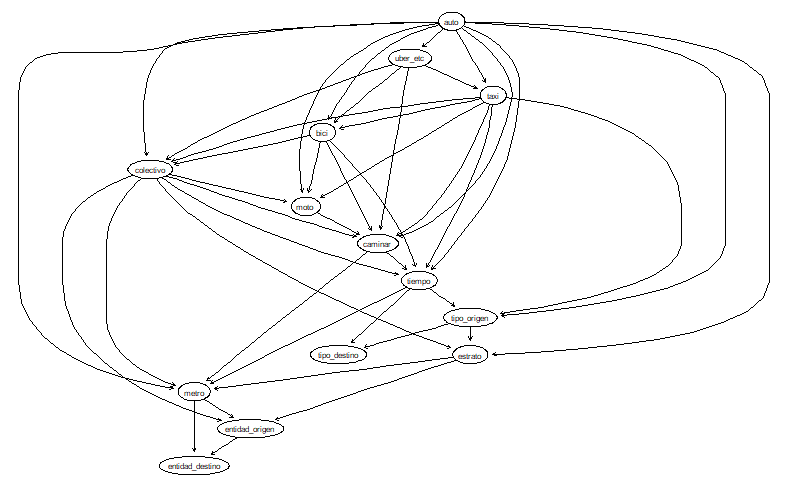
\includegraphics[width=0.5\textwidth]{dag_hc.png}
    \caption{Estructura DAG generada utilizando un algoritmo hill-climbing.}
\end{figure}

\begin{figure}[h!]
\centering
\resizebox{0.5\textwidth}{!}{
\begin{tabular}{|c|c|c|}
\hline
\textbf{DAG} & \textbf{Puntaje BIC} & \textbf{Puntaje AIC} \\ \hline
A        & -6916796 & -5722651 \\ \hline
B        & -6223229 & -5602247 \\ \hline
C        & -5544626 & -5528259 \\ \hline
HC       & -4653180 & -4620061 \\ \hline

\end{tabular}
}
\caption{Puntajes BIC y AIC para cada estructura DAG planteada.}
\label{fig:tabla_top10}
\end{figure}

Al final se seleccionó la DAG que maximiza el puntaje BIC, aquella realizada utilizando hill-climbing, con la cual se brindó solución a las consultas ya mencionadas.

\section{Resultados}
Al hacer las consultas en la red correspondiente, se obtienen los siguientes resultados:

\begin{itemize}
    \item La probabilidad estimada de que el tiempo de viaje sea menor a 20 minutos dado que el medio de transporte fue un automóvil es igual a $P=0.3195917$.
    
    \item  La probabilidad estimada de que un viaje en la Ciudad de México sea caminando o en bicicleta es de $P=0.6171179$.
    
    \item La probabilidad de que un hogar de estrato medio bajo utilice más de dos medios de transporte diferentes es de $P=0.07379346$.

    \item La probabilidad de que un viaje del hogar a la escuela dure más de 60 minutos dado que la persona viaja en auto es de $P=0.05340155$.
    
\end{itemize}

Los resultados obtenidos son satisfactorios. La probabilidad de que un hogar de estrato medio bajo utilice más de dos medios de transporte diferentes es apenas del $7\%$, lo cual resulta significativo si consideramos que en este cálculo se incluyen opciones como caminar o usar bicicleta. Este dato refleja las limitaciones y complicaciones que enfrentan muchas familias para trasladarse, evidenciando desigualdades estructurales en el acceso a opciones de movilidad eficientes. En contraste, el hecho de que aproximadamente el $61\%$ de los viajes en la Ciudad de México se realicen a pie o en bicicleta puede interpretarse de dos maneras: por un lado, podría indicar un diseño urbano que facilita y promueve la movilidad no motorizada; por otro, podría reflejar que una gran parte de la población se ve obligada a transportarse de esta forma debido a restricciones económicas o a la falta de alternativas accesibles.

\section{Conclusiones}
Las redes bayesianas multinomiales son útiles para modelar, entender y evaluar la relación entre los diferentes factores de diversas situaciones. En este estudio, las redes bayesianas probaron ser una manera de entender cómo los tiempos de viaje, las decisiones de transporte y las circunstancias de la población se relacionan entre sí. La DAG resultante permite estimar probabilidades condicionales de escenarios diversos y analizar resultados en base al estado de la vialidad de la zona. Permite cuantificar el impacto de múltiples factores como los tiempos de trayecto, el uso de diferentes medios de transporte, los destinos de la población, dándonos acceso a una imagen completa de cómo y por qué se transportan las personas dentro de la Zona Metropolitana del Valle de México.

En conjunto, estos datos vistos a través de la red proporcionan una herramienta importante al momento de tomar decisiones en temas de planeación urbana, ya que nos permiten explorar diferentes escenarios y predecir cómo estos pueden afectar otra parte completamente diferente del sistema de transporte. Por ejemplo, podemos saber si es plausible hacer cambios para mejorar el transporte público en ciertas zonas de la ciudad donde el trayecto es muy tardado, o mejorar vías específicas como el viaje por motocicleta o bicicleta. 

Este estudio no identifica la causalidad de manera directa; por ello, la información que proporciona debe interpretarse con cautela y complementarse con un análisis más amplio en materia de urbanismo, así como con una revisión precisa para cada consulta. Debemos ser prudentes con las conclusiones a las que nos conducen los resultados, ya que no estamos tomando en cuenta varios aspectos como las calles transitadas o la temporalidad de los datos. Estas son algunas de las consideraciones que se tienen que tener al replicar este estudio o aplicarlo en escenarios reales.

% Include references
\insertbibliography{References}

\end{document}
